\newpage
\section{Dreidimensionales Punktediagramm}

Falls Datensätze mit einer unabhängigen und zwei abhängigen Variablen dargestellt werden sollen, kann ein dreidimensionales Punktediagramm verwendet werden.

Beispiele für Datensätze, die in dreidimensionalen Punktediagrammen dargestellt werden können:

\begin{itemize}
	\item Zwei Attribute im Laufe der Zeit, zum Beispiel BIP und Anstellung eines Landes
	\item Drei Attribute, die in einem bestimmten Verhältnis zueinander stehen. Zum Beispiel Geschwindigkeit, Luftwiderstand, Oberfläche
\end{itemize}

Es wurde entschieden, eine weitere Applikation zu entwickeln, die einen Datensatz mit einer unabhängigen und zwei abhängigen Variablen in einer 3D-Applikation anzeigt.

\subsection{Applikation}

\begin{figure}[H]
	\centering
	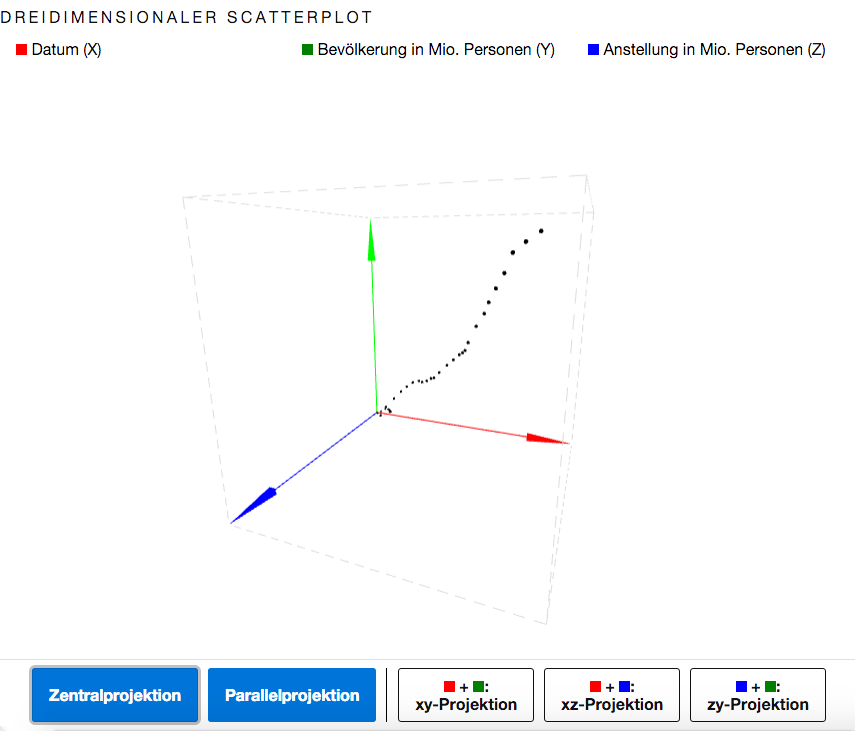
\includegraphics[width=\linewidth]{images/3d}
	\caption{Oberfläche der Applikation (dreidimensionales Punktediagramm), perspektivische Projektion}
	\label{fig:3d}
\end{figure}

Die Applikation wurde mit der Programmierbibliothek \textit{Three.js} \cite{threejs} erstellt. Three.js ermöglicht die Entwicklung von 3D-Applikationen mit JavaScript im Browser.

\textbf{Achsen.} Als Achsen wurden verschiedenfarbige Pfeile (Abbildung \ref{fig:vectors}) mit Richtungsvektoren $\vec{a}_x$, $\vec{a}_y$, $\vec{a}_z$ erstellt.

\begin{figure}[H]
	\centering
	$\vec{a}_x=\begin{pmatrix} 1 \\ 0 \\ 0 \end{pmatrix}$ (rot)\qquad
	$\vec{a}_y=\begin{pmatrix} 0 \\ 1 \\ 0 \end{pmatrix}$ (grün)\qquad
	$\vec{a}_z=\begin{pmatrix} 0 \\ 0 \\ 1 \end{pmatrix}$ (blau)\qquad
	\caption{Die Richtungsvektoren der Achsen im dreidimensionalen Punktediagramm.}
	\label{fig:vectors}
\end{figure}

Die Beschriftung und Farben der Achsen werden über dem Diagramm angezeigt. Die erste Beschriftung (rot) steht für die unabhängige Variable, die zweite und dritte Beschriftung für die abhängigen Variablen.

\textbf{Punkte.} Die Datenpunkte wurden an den drei Achsen abgetragen und als schwarze Kugeln im Raum abgebildet.

\textbf{Würfel.} Ein Würfel wurde mit gestrichelten grauen Linien um das Diagramm dargestellt. Es soll dem Nutzer helfen, sich in dem dreidimensionalen Raum zu orientieren.

\textbf{Rotation.} Das dreidimensionale Punktediagramm ist mit der Maus rotierbar. Die Kamera bleibt während der Rotation stets auf die Mitte des Diagramms gerichtet. Die Rotation ermöglicht eine bessere Erkundung des Datensatzes und bietet die Ansicht aus verschiedenen Winkeln dar.

Eine Funktion für das Zommen wurde nicht implementiert, weil sie sich als kontraproduktiv herausstellte: Die Orientation des Benutzers geht schnell verloren, zum Beispiel wenn zu weit herausgezoomt wird, sodass das Diagramm nicht mehr sichtbar ist, oder wenn sich die Kamera innerhalb der Punktewolke befindet.

\subsection{Projektion des Diagramms}

Eine besondere Erkenntnis bei der Entwicklung dieser Applikation ist das Potential von orthographischen Projektionen innerhalb des dreidimensionalen Punktediagramms.

Das Punktediagramm kann durch Verschieben der Kamera und Verwendung der orthographischen Projektion auf ein zweidimensionales Punktediagramm reduziert werden.

Die Projektion der XY-Fläche kann zum Beispiel erzielt werden, wenn die Kamera auf halber X-Achsen-Position, halber Y-Achsen-Position und auf doppelter Z-Achsen-Position ist und in die Richtung der Mitte des Diagrammes ausgerichtet ist.

\begin{figure}[H]

	$S = (0|0|0)$
	
	$M = (\frac{1}{2} a | \frac{1}{2} a | \frac{1}{2} a)$
	
	$P_{xy} = (\frac{1}{2} a | \frac{1}{2} a| a + a)$
	
	$P_{yz} = (\frac{1}{2} a | -a| \frac{1}{2} a)$
	
	$P_{zx} = (-a | \frac{1}{2} a| \frac{1}{2} a)$
\end{figure}

\begin{figure}[!htbp]
	\centering
	\begin{minipage}{.45\textwidth}
		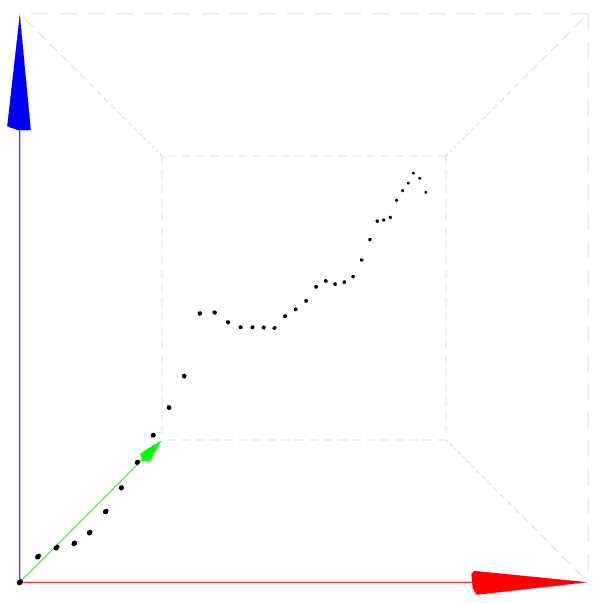
\includegraphics[width=\linewidth]{images/persp}
	\end{minipage}
	\begin{minipage}{.45\textwidth}
		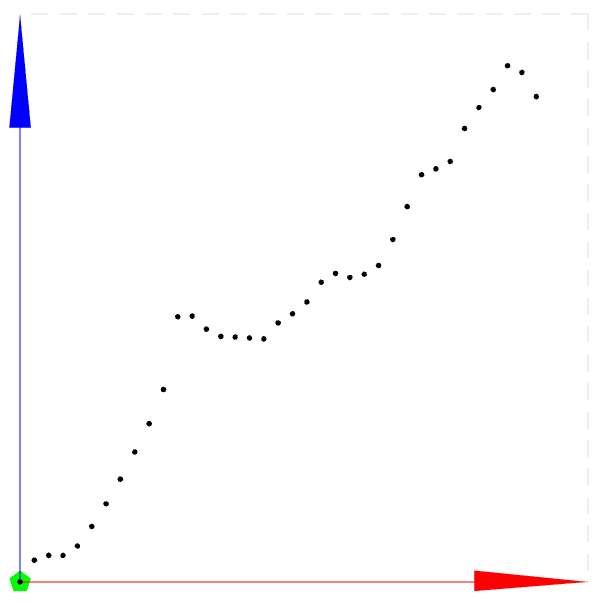
\includegraphics[width=\linewidth]{images/ortho}
	\end{minipage}
	\caption[cap]{cap}
	\label{fig:projections}
\end{figure}